\section{Results}

\subsection{Q1a: in-domain pragmatic performance}

\begin{figure*}[t]
  \centering
  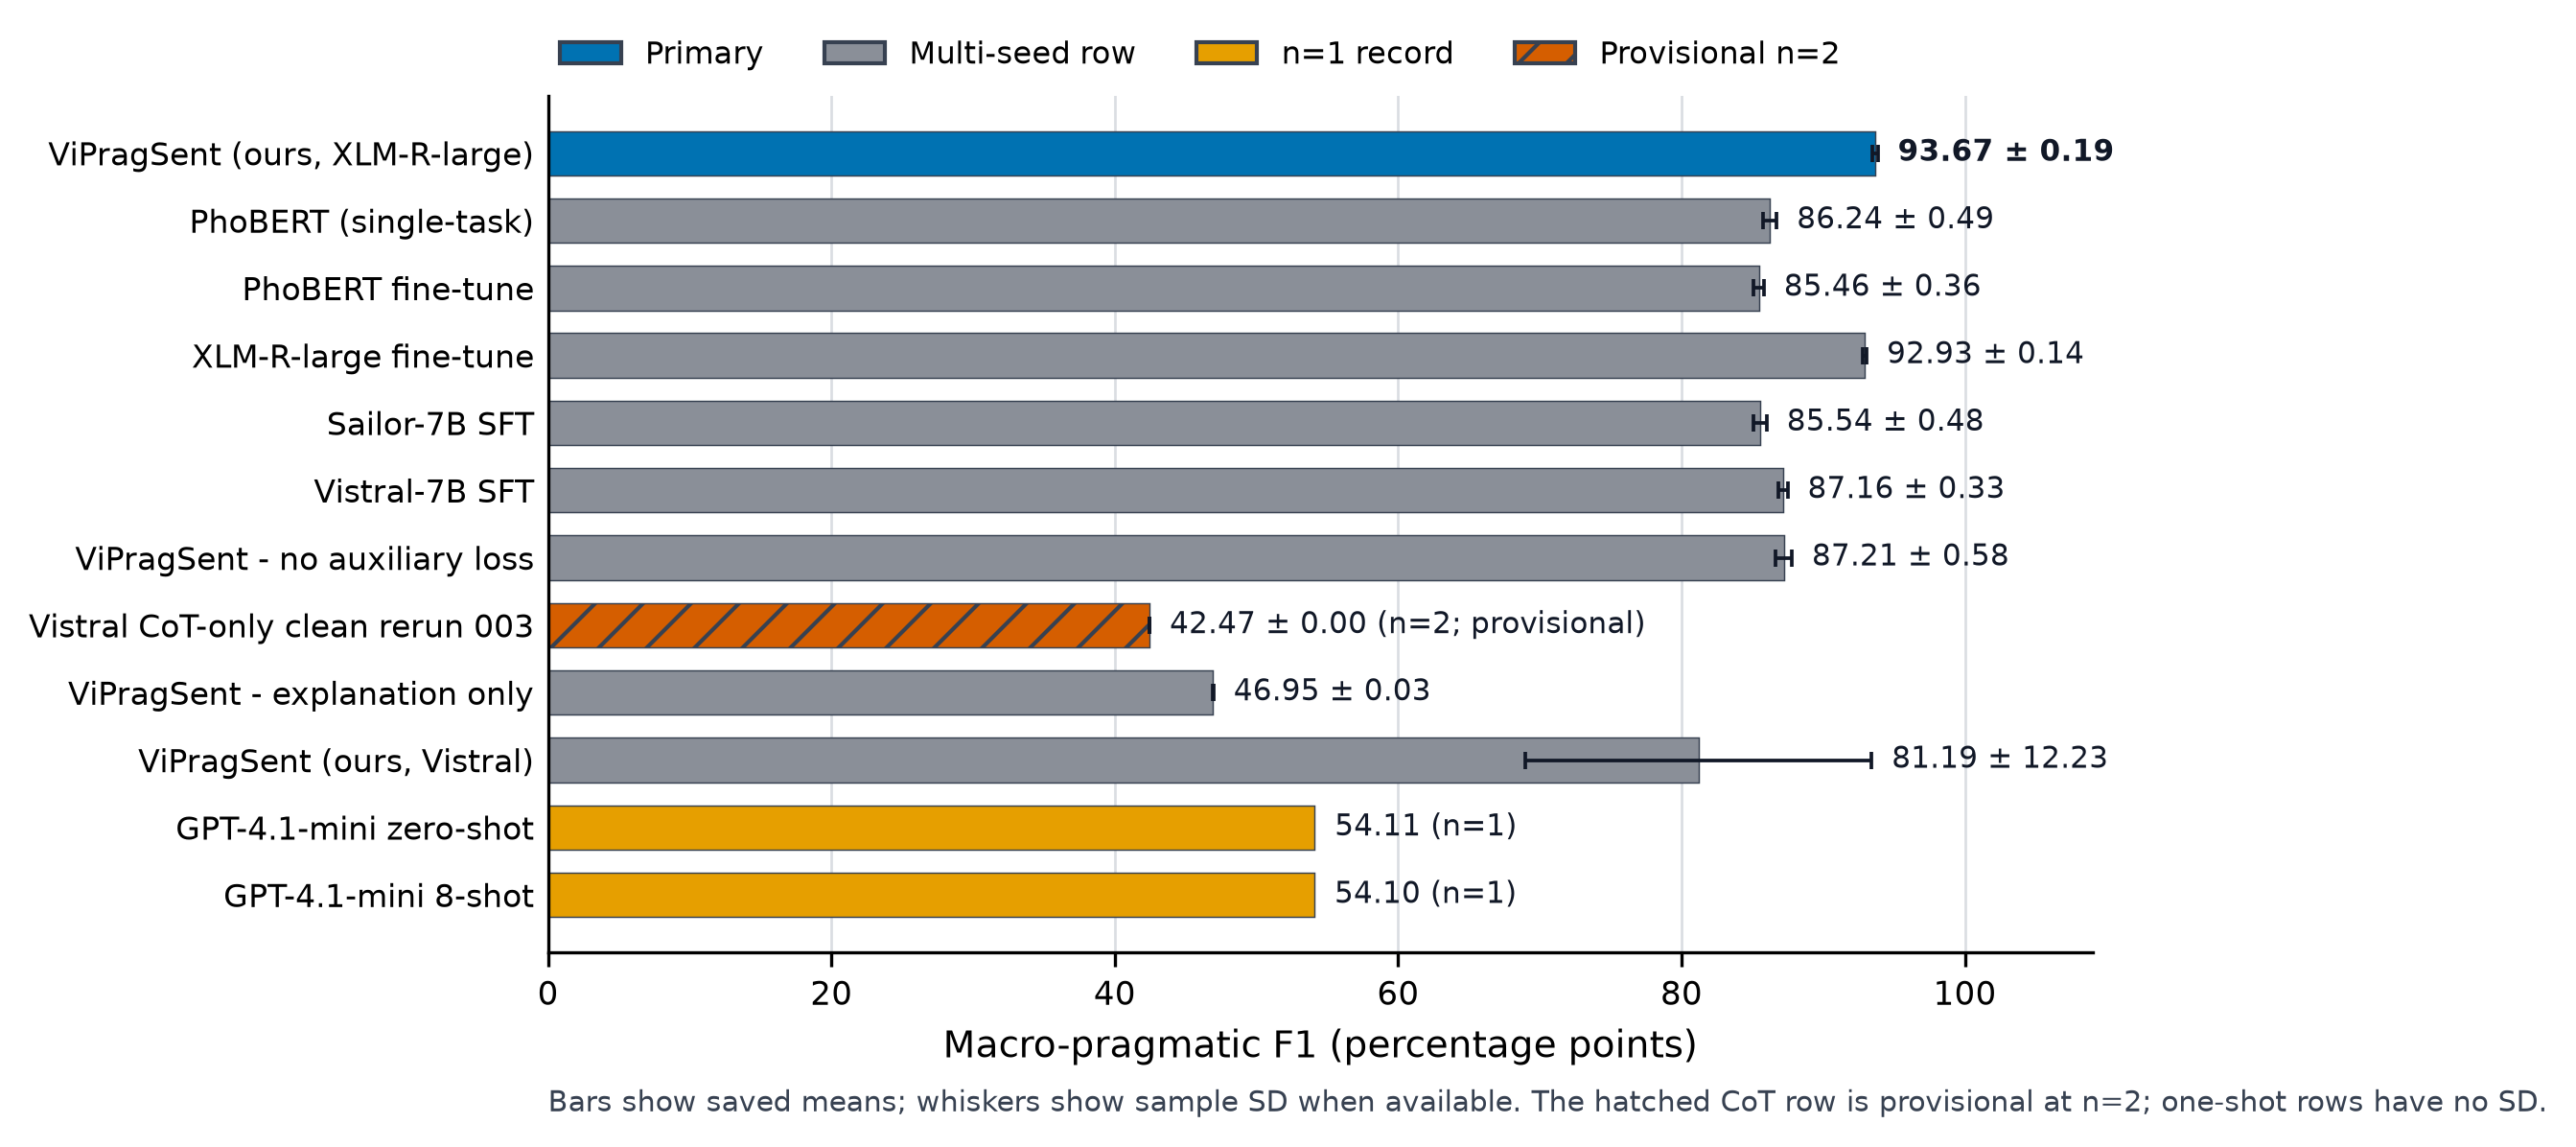
\includegraphics[width=\textwidth]{figures/figure_q1a_table_macro_bars.png}
  \caption{Q1a macro-pragmatic F1 across the expanded rows in Table~\ref{tab:q1a}. Bars show saved means on the 0--100 percentage-point scale; whiskers show sample SD when a multi-seed estimate is available. Complete three-seed rows are directly comparable for the primary baseline claim; one-shot reference records and the provisional $n=2$ CoT record are retained for coverage and are not treated as complete three-seed baselines.}
  \label{fig:q1a-table-bars}
\end{figure*}

Table 1 gives the expanded canonical Q1a result with systems as rows and the six pragmatic metrics plus their macro average as columns. Values are mean $\pm$ sample SD in percentage points. The target remains highest in mean on every metric among the five complete three-seed baseline families; the other rows are contextual variants, provisional coverage, or one-shot records as marked in the caption and the machine-readable canonical row ledger.

\begin{table*}[t]
\centering
\scriptsize
\setlength{\tabcolsep}{1.5pt}
\begin{tabularx}{\textwidth}{>{\raggedright\arraybackslash}p{1.55in} >{\centering\arraybackslash}X >{\centering\arraybackslash}X >{\centering\arraybackslash}X >{\centering\arraybackslash}X >{\centering\arraybackslash}X >{\centering\arraybackslash}X >{\centering\arraybackslash}X}
\hline
\shortstack[l]{Model} & \shortstack[l]{Implicit\\sentiment} & Sarcasm & Irony & \shortstack[l]{Idiom/\\figurative} & \shortstack[l]{Code-\\switching} & Mocking & \shortstack[l]{Macro-pragmatic\\F1} \\
\hline
ViPragSent (ours, XLM-R-large) & \mbox{92.67 $\pm$ 0.24} & \mbox{89.36 $\pm$ 0.90} & \mbox{98.43 $\pm$ 0.20} & \mbox{93.35 $\pm$ 0.66} & \mbox{94.84 $\pm$ 0.56} & \mbox{93.35 $\pm$ 0.73} & \textbf{\mbox{93.67 $\pm$ 0.19}} \\
PhoBERT (single-task) & \mbox{88.00 $\pm$ 1.29} & \mbox{70.87 $\pm$ 1.34} & \mbox{97.13 $\pm$ 1.06} & \mbox{91.21 $\pm$ 0.78} & \mbox{91.08 $\pm$ 1.51} & \mbox{79.16 $\pm$ 2.99} & \mbox{86.24 $\pm$ 0.49} \\
PhoBERT fine-tune & \mbox{85.76 $\pm$ 0.72} & \mbox{72.64 $\pm$ 0.50} & \mbox{97.45 $\pm$ 0.19} & \mbox{86.63 $\pm$ 0.66} & \mbox{91.73 $\pm$ 0.53} & \mbox{78.53 $\pm$ 1.01} & \mbox{85.46 $\pm$ 0.36} \\
XLM-R-large fine-tune & \mbox{92.16 $\pm$ 0.13} & \mbox{88.12 $\pm$ 0.43} & \mbox{97.93 $\pm$ 0.10} & \mbox{92.85 $\pm$ 0.68} & \mbox{94.27 $\pm$ 0.04} & \mbox{92.27 $\pm$ 0.41} & \textbf{\mbox{92.93 $\pm$ 0.14}} \\
Sailor-7B SFT & \mbox{85.42 $\pm$ 0.27} & \mbox{72.14 $\pm$ 2.96} & \mbox{95.75 $\pm$ 0.52} & \mbox{91.15 $\pm$ 1.40} & \mbox{91.03 $\pm$ 0.74} & \mbox{77.76 $\pm$ 1.21} & \mbox{85.54 $\pm$ 0.48} \\
Vistral-7B SFT & \mbox{87.36 $\pm$ 0.31} & \mbox{74.74 $\pm$ 0.94} & \mbox{96.69 $\pm$ 0.23} & \mbox{91.48 $\pm$ 1.55} & \mbox{92.80 $\pm$ 0.60} & \mbox{79.91 $\pm$ 0.26} & \mbox{87.16 $\pm$ 0.33} \\
ViPragSent - no auxiliary loss & \mbox{87.43 $\pm$ 0.62} & \mbox{74.79 $\pm$ 0.53} & \mbox{97.15 $\pm$ 0.27} & \mbox{91.51 $\pm$ 0.99} & \mbox{92.88 $\pm$ 0.63} & \mbox{79.51 $\pm$ 2.81} & \mbox{87.21 $\pm$ 0.58} \\
Vistral CoT-only clean rerun 003 (2/3) & \mbox{17.36 $\pm$ 0.00} & \mbox{48.24 $\pm$ 0.00} & \mbox{48.20 $\pm$ 0.00} & \mbox{48.17 $\pm$ 0.00} & \mbox{45.92 $\pm$ 0.00} & \mbox{46.91 $\pm$ 0.00} & \mbox{42.47 $\pm$ 0.00} \\
ViPragSent - explanation only & \mbox{44.13 $\pm$ 0.00} & \mbox{48.24 $\pm$ 0.00} & \mbox{48.20 $\pm$ 0.00} & \mbox{48.17 $\pm$ 0.00} & \mbox{46.02 $\pm$ 0.18} & \mbox{46.91 $\pm$ 0.00} & \mbox{46.95 $\pm$ 0.03} \\
ViPragSent (ours, Vistral) & \mbox{84.93 $\pm$ 5.49} & \mbox{72.59 $\pm$ 7.73} & \mbox{94.75 $\pm$ 3.18} & \mbox{79.38 $\pm$ 22.13} & \mbox{78.36 $\pm$ 26.44} & \mbox{77.15 $\pm$ 8.60} & \mbox{81.19 $\pm$ 12.23} \\
GPT-4.1-mini zero-shot & 45.44 (n=1) & 56.51 (n=1) & 53.17 (n=1) & 52.45 (n=1) & 62.42 (n=1) & 54.69 (n=1) & 54.11 (n=1) \\
GPT-4.1-mini 8-shot & 49.04 (n=1) & 61.09 (n=1) & 52.37 (n=1) & 50.87 (n=1) & 56.89 (n=1) & 54.32 (n=1) & 54.10 (n=1) \\
\hline
\end{tabularx}
\caption{Q1a in-domain pragmatic performance on the 2,000-example ID/gold test split. Systems are rows; the six pragmatic metrics and macro-pragmatic F1 are columns. The primary row is ViPragSent (ours, XLM-R-large). Entries are mean $\pm$ sample SD from the compact canonical rows; n=1 rows have no SD and the CoT row is provisional at n=2. Canonical row statuses are retained in the machine-readable q1a-extra ledger.}
\label{tab:q1a}
\end{table*}

Against the strongest complete baseline, the observed mean gaps are +0.51 pp for implicit sentiment, +1.24 pp for sarcasm, +0.50 pp for irony, +0.50 pp for idiom/figurative language, +0.57 pp for code-switching, and +1.07 pp for mocking. The two largest observed head gaps are therefore sarcasm and mocking, but these are descriptive differences across saved predictions, not significance claims. The macro difference is 93.665838 - 92.934251 = +0.731587 percentage points, reported as +0.73 pp.

The expanded remote candidate coverage remains in Appendix B. The canonical row status fields are retained in the machine-readable ledger, and the two cohorts are kept separate because the report has a different cohort for some rows; its bootstrap confidence-interval half-widths are not used as sample SD.

\subsection{Q1b: external retention}
Table 2 expands Q1b using the canonical external-retention artifact. It shows mixed transfer rather than uniformly preserved performance: the primary is not the highest ordinary-F1 record in this analyzed set, and its per-dataset profile differs from the classification baselines. The table retains the actual saved recipe names for the six comparable three-seed records and adds the complete three-seed PhoBERT-backed ViPragSent inventory as a contextual variant. The contextual row is not the primary model and is not a substitute for a reference-row recipe. The identity-mismatched Azure deployment and unresolved GPT-4o-mini 8-shot record remain in the machine-readable audit ledger and are not printed as manuscript rows.

\begin{table*}[t]
\centering
\scriptsize
\setlength{\tabcolsep}{2pt}
\begin{tabularx}{\textwidth}{>{\raggedright\arraybackslash}p{1.55in} >{\raggedleft\arraybackslash}p{0.85in} >{\raggedleft\arraybackslash}p{0.85in} >{\raggedleft\arraybackslash}p{0.85in} >{\raggedleft\arraybackslash}p{0.85in}}
\hline
\shortstack[l]{Model record} & \shortstack[l]{UIT-\\VSFC} & \shortstack[l]{UIT-\\VSMEC} & \shortstack[l]{AIVIVN-human-\\derived-3way} & \shortstack[l]{Ordinary\\F1} \\
\hline
PhoBERT single-task routed & \mbox{29.7 $\pm$ 0.5} & \mbox{38.8 $\pm$ 1.5} & \mbox{45.4 $\pm$ 2.6} & \mbox{38.0 $\pm$ 0.3} \\
PhoBERT multitask 8-head & \mbox{33.6 $\pm$ 3.0} & \mbox{36.4 $\pm$ 0.7} & \mbox{44.7 $\pm$ 1.3} & \mbox{38.2 $\pm$ 1.5} \\
XLM-R-large multitask 8-head & \mbox{39.1 $\pm$ 1.1} & \mbox{40.2 $\pm$ 0.2} & \mbox{48.3 $\pm$ 1.2} & \mbox{42.5 $\pm$ 0.5} \\
ViPragSent (ours, XLM-R-large) & \mbox{37.9 $\pm$ 2.8} & \mbox{40.0 $\pm$ 0.7} & \mbox{47.9 $\pm$ 2.2} & \mbox{42.0 $\pm$ 1.8} \\
ViPragSent full PhoBERT inventory (contextual) & \mbox{34.1 $\pm$ 0.7} & \mbox{36.0 $\pm$ 0.3} & \mbox{45.5 $\pm$ 0.8} & \mbox{38.6 $\pm$ 0.5} \\
Sailor-7B SFT & \mbox{34.4 $\pm$ 3.2} & \mbox{40.7 $\pm$ 0.7} & \mbox{48.7 $\pm$ 1.4} & \mbox{41.3 $\pm$ 1.2} \\
Vistral-7B SFT & \mbox{30.7 $\pm$ 6.4} & \mbox{39.4 $\pm$ 1.5} & \mbox{49.0 $\pm$ 0.8} & \mbox{39.7 $\pm$ 2.5} \\
\hline
\end{tabularx}
\caption{External retention on the UIT-VSFC, UIT-VSMEC, and AIVIVN test cohorts. The primary row is ViPragSent (XLM-R-large); the PhoBERT-backed inventory row is contextual rather than primary. Entries are mean $\pm$ sample SD over three saved runs. Columns report macro-F1 in percentage points and their unweighted ordinary-F1 aggregate.}
\label{tab:q1b}
\end{table*}

All entries in the main table are mean plus/minus sample SD over three saved runs, including the contextual inventory row. The external datasets differ in domain and target semantics, so the table is a retention profile rather than a single generalization score. The primary-versus-standard descriptive comparison has observed ID/gold/raw-text/ NFC parity on all three evaluated cohorts, while the AIVIVN source-manifest hash discrepancy remains a provenance limitation; no full-row ordinary-F1 superiority claim is made.

The canonical recipe ledger is retained separately from the metric table: \texttt{phobert\_pol\_single} + \texttt{phobert\_emo\_single} for PhoBERT single-task routed; \texttt{phobert\_multitask\_8head}; \texttt{xlmr\_multitask\_8head}; \texttt{xlmr\_followup\_full} for the primary; \texttt{sailor\_multitask\_8head}; \texttt{vistral\_multitask\_8head}; and \texttt{azure\_gpt41\_mini} dedicated prompts for the actual GPT-4.1-mini deployment.

\subsection{Q2: auxiliary-task and uncertainty ablations}
Table 3 reports the separate XLM-R follow-up cohort. Within this cohort, the full configuration is not the highest reported macro-pragmatic F1: removing task-uncertainty weighting gives 92.9 versus 92.8 for the full configuration. The full configuration has lower reported ECE than the no-uncertainty variant, while removing the explanation auxiliary reduces relative cost substantially and changes F1 and ECE. Removing the multitask bundle causes a much larger F1 reduction. These are trade-offs within Q2, not evidence that one component is universally beneficial.

For compactness, Table 3 labels the variants as Full, $-$ emotion, $-$ explanation, Single-task bundle, $-$ polarity, and $-$ uncertainty; these mean the full follow-up, removal of the named auxiliary or weighting component, and the no-multitask component bundle, respectively.

\begin{table*}[t]
\centering
\scriptsize
\setlength{\tabcolsep}{2pt}
\begin{tabularx}{\textwidth}{>{\raggedright\arraybackslash}X >{\raggedleft\arraybackslash}r >{\raggedleft\arraybackslash}r >{\raggedleft\arraybackslash}r}
\hline
XLM-R variant & Macro-pragmatic F1 & Polarity dev ECE (x10\textsuperscript{3}) & Relative cost \\
\hline
Full & \mbox{92.8 $\pm$ 0.6} & \mbox{81.1 $\pm$ 11.7} & 1.00 \\
- emotion & \mbox{91.7 $\pm$ 0.7} & \mbox{56.2 $\pm$ 22.5} & 0.65 \\
- explanation & \mbox{92.3 $\pm$ 1.3} & \mbox{68.1 $\pm$ 22.2} & 0.20 \\
Single-task bundle & \mbox{74.7 $\pm$ 2.3} & \mbox{118.9 $\pm$ 69.1} & 1.10 \\
- polarity & \mbox{92.8 $\pm$ 0.2} & not applicable & 0.81 \\
- uncertainty & \mbox{92.9 $\pm$ 0.3} & \mbox{90.2 $\pm$ 5.9} & 0.82 \\
\hline
\end{tabularx}
\caption{Q2 follow-up ablations. Macro-pragmatic F1 is evaluated on the Q2 test split; polarity ECE is the verified development-split ten-bin top-label ECE, shown on the x10$^3$ scale. The legacy field name is \texttt{polarity\_dev\_ece}; the no-polarity row is not applicable because its polarity head was removed. Entries are mean $\pm$ sample SD over $n=3$ runs.}
\label{tab:q2}
\end{table*}

Note: For all three no-polarity seeds, ECE is not applicable because the polarity head was removed; no polarity probability source exists. Table 3 uses the current Q2 protocol: ten-bin top-label ECE from the saved development metrics and predictions, reported on the $10^3$ scale. The legacy field name \texttt{polarity\_dev\_ece} is retained for provenance. This is not Q4's six-head calibration metric. The no-multitask entry is a separate single-task component-bundle recipe. Because Q2 is a separate cohort, its scientific comparison is the pattern across named variants, not an explanation of Q1a's absolute score.

\subsection{Q3: pragmatic label-budget behavior}

\begin{figure}[t]
  \centering
  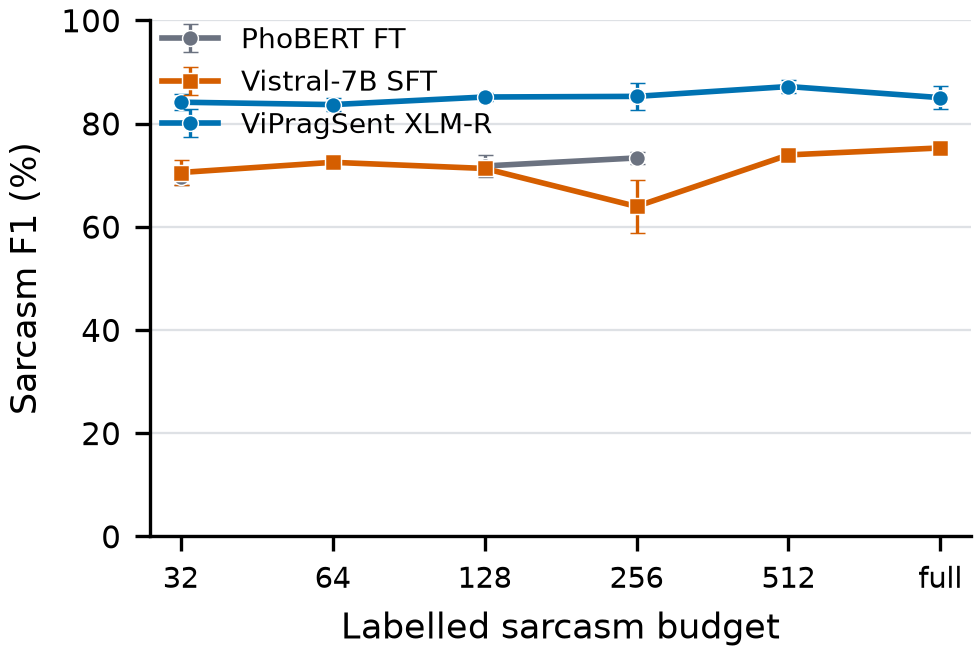
\includegraphics[width=\columnwidth]{figures/figure_q3_sarcasm_budget.png}
  \caption{Q3 sarcasm F1 across pragmatic-label budgets. Curves show artifact-derived means and sample SD over three logical runs where the cohort is complete ($n=3$; run labels 21, 22, and 23, corresponding to remote artifact seeds 20260521, 20260522, and 20260523). The PhoBERT curve has gaps at 64, 512, and full because those standard-GPU40 cells lack complete three-seed test evidence. The target is shown with PhoBERT fine-tune and Vistral-7B SFT for context.}
  \label{fig:q3-sarcasm-budget}
\end{figure}

Table 4 reports the XLM-R follow-up budget profile together with contextual PhoBERT and Vistral baseline curves. Complete entries are mean $\pm$ sample SD over three runs. Thresholds are tuned on the fixed development split; the displayed metrics are evaluated on the fixed test split. The standard GPU40 PhoBERT cohort has complete three-seed evidence only at 32, 128, and 256 positives; its 64, 512, and full-budget cells are not imputed. A separate compact-final PhoBERT cohort is documented in \texttt{figures/\allowbreak{}source\_d\allowbreak{}ata/q3\_p\allowbreak{}hobert\_c\allowbreak{}ohort\_au\allowbreak{}dit.md} but is not mixed into this table because its 32 and 128 aggregates differ.

\begin{table*}[t]
\centering
\small
\setlength{\tabcolsep}{3pt}
\begin{tabularx}{\textwidth}{>{\raggedright\arraybackslash}X >{\raggedright\arraybackslash}X >{\raggedright\arraybackslash}X >{\raggedright\arraybackslash}X}
\hline
Positive examples & ViPragSent (XLM-R-large) sarcasm / macro & PhoBERT (fine-tune) sarcasm / macro & Vistral-7B SFT sarcasm / macro \\
\hline
32 & 84.2 $\pm$ 1.6 / 91.1 $\pm$ 1.3 & 69.7 $\pm$ 1.5 / 84.2 $\pm$ 0.7 & 70.5 $\pm$ 2.4 / 86.2 $\pm$ 0.2 \\
64 & 83.7 $\pm$ 1.3 / 91.2 $\pm$ 0.8 & -- & 72.5 $\pm$ 0.9 / 86.7 $\pm$ 0.5 \\
128 & 85.2 $\pm$ 0.7 / 91.6 $\pm$ 0.2 & 71.8 $\pm$ 2.2 / 84.0 $\pm$ 1.2 & 71.3 $\pm$ 0.6 / 86.2 $\pm$ 0.4 \\
256 & 85.3 $\pm$ 2.6 / 91.6 $\pm$ 1.2 & 73.4 $\pm$ 1.2 / 84.5 $\pm$ 0.9 & 64.0 $\pm$ 5.1 / 70.3 $\pm$ 14.2 \\
512 & 87.2 $\pm$ 1.2 / 92.3 $\pm$ 0.7 & -- & 73.9 $\pm$ 1.2 / 87.2 $\pm$ 0.3 \\
Full & 85.0 $\pm$ 2.3 / 91.1 $\pm$ 1.3 & -- & 75.3 $\pm$ 0.8 / 87.4 $\pm$ 0.2 \\
\hline
\end{tabularx}
\caption{Q3 pragmatic label-budget behavior on the fixed test split, using the three available systems in \texttt{figures/source\_data/table\_q3\_low\_resource.csv}: ViPragSent (XLM-R-large), PhoBERT (fine-tune), and Vistral-7B SFT. Complete entries are mean $\pm$ sample SD over $n=3$ logical runs; -- denotes PhoBERT cells without a complete three-seed test cohort and is not imputed. The separate compact-final PhoBERT cohort is not mixed with the standard GPU40 cohort.}
\label{tab:q3}
\end{table*}

ViPragSent (XLM-R-large) exceeds the complete PhoBERT baseline rows at the budgets where that cohort is available. Its curves are non-monotonic: macro-pragmatic F1 rises from 91.1 at 32 positives to 92.3 at 512 and returns to 91.1 at full budget. Missing 64/512/full PhoBERT cells limit the contextual baseline curve. This is a sample-efficiency diagnostic, not evidence that less data is generally preferable; the supplied plot visualizes the same cohort.

\subsection{Q4: calibration}

\begin{figure}[t]
  \centering
  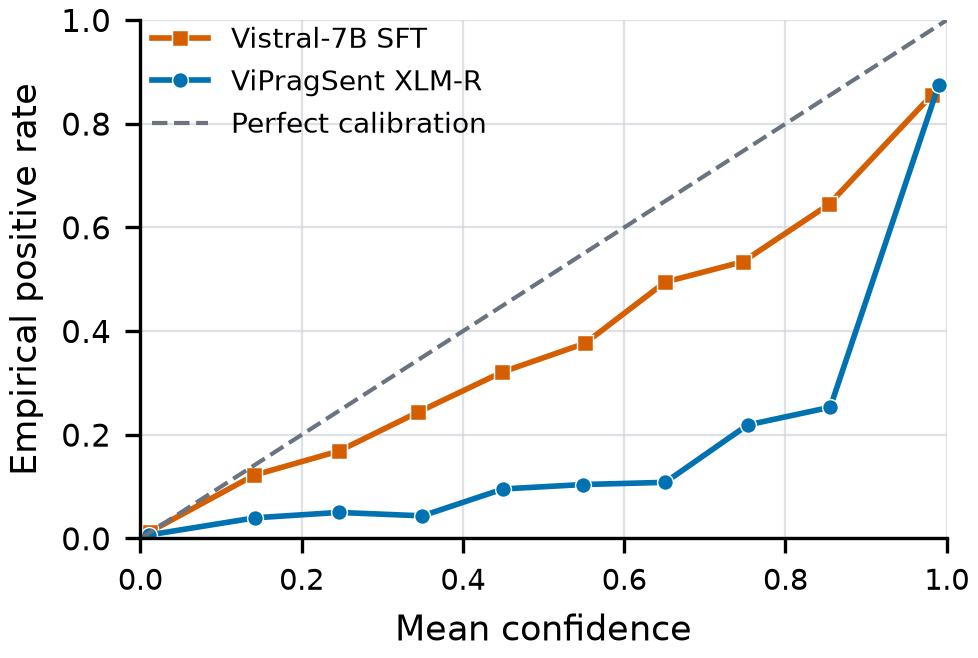
\includegraphics[width=\columnwidth]{figures/figure_q4_reliability.png}
  \caption{Q4 reliability diagrams for the calibration comparison. Curves aggregate the supplied per-label reliability bins over three logical runs ($n=3$; run labels 21, 22, and 23, corresponding to remote artifact seeds 20260521, 20260522, and 20260523). The dashed line denotes perfect calibration; the figure is descriptive and does not imply target dominance.}
  \label{fig:q4-reliability}
\end{figure}

Under the Q4 extraction protocol, the ViPragSent XLM-R target has ECE 0.0386 $\pm$ 0.0069, while the Vistral comparison record has ECE 0.0345 $\pm$ 0.0041. Lower ECE is better, so the comparison does not support target calibration dominance. Q4 extracts raw positive sigmoid probabilities from same-seed Q1a v37 checkpoints without retraining; ECE depends on its split, ten bins, and probability source.
